% Created 2015-02-07 sáb 18:50
\documentclass[xcolor={usenames,svgnames,dvipsnames}]{beamer}
\usepackage[utf8]{inputenc}
\usepackage[T1]{fontenc}
\usepackage{fixltx2e}
\usepackage{graphicx}
\usepackage{longtable}
\usepackage{float}
\usepackage{wrapfig}
\usepackage{rotating}
\usepackage[normalem]{ulem}
\usepackage{amsmath}
\usepackage{textcomp}
\usepackage{marvosym}
\usepackage{wasysym}
\usepackage{amssymb}
\usepackage{hyperref}
\tolerance=1000
\usepackage{color}
\usepackage{listings}
\usepackage{mathpazo}
\usepackage{gensymb}
\usepackage{amsmath}
\bibliographystyle{plain}
\AtBeginSubsection[]{\begin{frame}[plain]\tableofcontents[currentsubsection,sectionstyle=show/shaded,subsectionstyle=show/shaded/hide]\end{frame}}
\AtBeginSection[]{\begin{frame}[plain]\tableofcontents[currentsection,hideallsubsections]\end{frame}}
\usepackage[emulate=units]{siunitx}
\sisetup{per=fraction, fraction=nice, decimalsymbol=comma}
\newunit{\wattpeak}{Wp}
\newunit{\watthour}{Wh}
\newunit{\amperehour}{Ah}
\hypersetup{colorlinks=true, linkcolor=Blue, urlcolor=Blue}
\setbeamercolor{alerted text}{fg=red!50!black} \setbeamerfont{alerted text}{series=\bfseries}
\usetheme[hideothersubsections]{Goettingen}
\usecolortheme{rose}
\usefonttheme{serif}
\author{Oscar Perpiñán Lamigueiro \\ \url{http://oscarperpinan.github.io}}
\date{}
\title{SFB: Diseño}
\hypersetup{
  pdfkeywords={},
  pdfsubject={},
  pdfcreator={Emacs 24.4.1 (Org mode 8.2.7c)}}
\begin{document}

\maketitle

\begin{frame}[label=sec-0-1]{}
\begin{center}
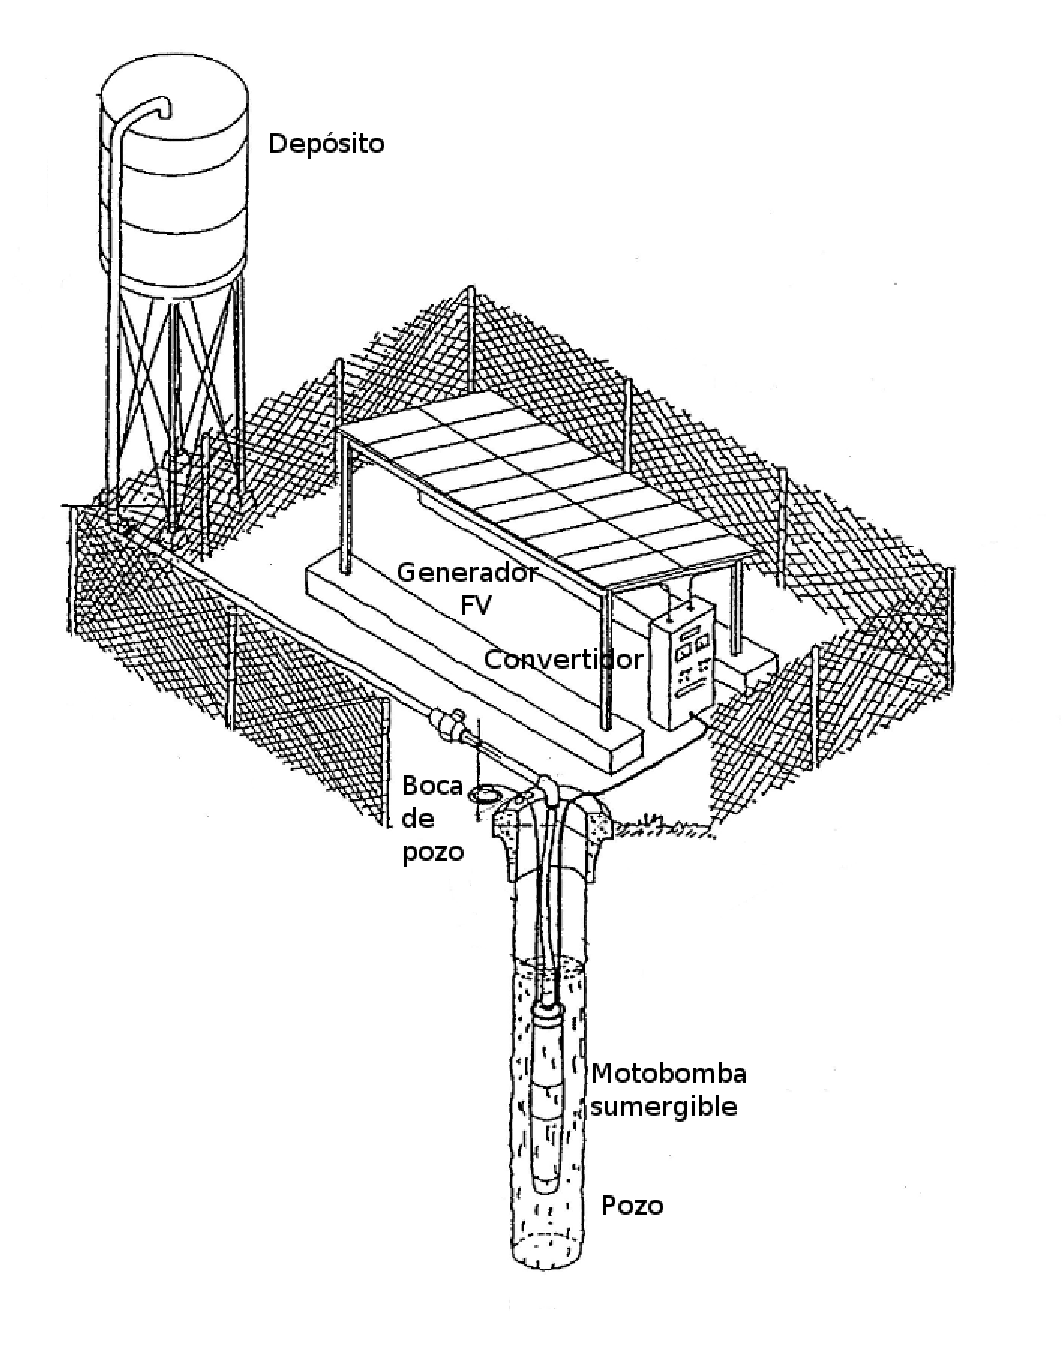
\includegraphics[height=0.9\textheight]{../figs/EsquemaBombeo_oscar.pdf}
\end{center}
\end{frame}


\section{Caudal}
\label{sec-1}


\begin{frame}[label=sec-1-1]{Potencia hidráulica}
\begin{itemize}
\item La \alert{potencia hidráulica}, $P_{H}$, necesaria para bombear agua es una función de, la \alert{altura vertical aparente}, $H_{v}$ y del \alert{caudal de agua}, $Q$:$$P_{H}=g\cdot\rho\cdot Q\cdot H_{v}$$ donde g es la aceleración de la gravedad, y $\rho$ es la densidad del agua.

\item Cambiando las unidades ($P_{H}$ en watios, $H_{v}$ en metros y $Q$ en $\si{\meter\cubed\per\hour}$)
\end{itemize}
$$P_{H}=2.725\cdot Q\cdot H_{V}$$
\end{frame}

\begin{frame}[label=sec-1-2]{Potencia eléctrica de la motobomba}
\begin{itemize}
\item Asumiendo que el agua bombeada sale por el conducto a una velocidad insignificante, la potencia de salida de la bomba necesita satisfacer $P_{H}$ más las \alert{perdidas de fricción en la tubería}, $P_{f}$.
\item La \alert{potencia eléctrica a la entrada de la motobomba} es ($\eta_{MP}$ es la \alert{eficiencia de la motobomba})
\end{itemize}
$$P_{el}=\frac{P_{H}+P_{f}}{\eta_{mp}}$$ 


\begin{itemize}
\item El valor de $P_{H}+P_{f}$ es la \alert{potencia mecánica a la salida de la bomba}. Este valor se asimila a una altura equivalente $H_{T}$ asociado a un caudal determinado:$$H_{T}=H_{v}+H_{f}$$
\end{itemize}
\end{frame}

\begin{frame}[label=sec-1-3]{Potencia eléctrica del generador}
La potencia eléctrica requerida por la motobomba es entregada por un generador FV y un acondicionador de potencia:$$P_{el}=P_{g}^{*}\cdot\frac{G}{G^{*}}\frac{\eta_{g}}{\eta_{g}^{*}}\cdot\eta_{inv}$$

siendo $\eta_{inv}$ la eficiencia del equipo de acondicionamiento de potencia.
\end{frame}



\begin{frame}[label=sec-1-4]{Caudal diario}
\begin{itemize}
\item El \alert{caudal diario} bombeado por este conjunto es: $$Q_{d}=\intop_{d}\frac{P_{g}^{*}\cdot\frac{G}{G^{*}}\frac{\eta_{g}}{\eta_{g}^{*}}\cdot\eta_{inv}\cdot\eta_{mp}}{2.725\cdot H_{T}}\mathrm{dt}$$

\item Debido a las variaciones de la temperatura ambiente y de la irradiancia, y también a causa del comportamiento dinámico de los pozos, \alert{todos los parámetros mencionados anteriormente varían a lo largo del tiempo}.

\item Integral no resoluble salvo por métodos numéricos (simulación)
\end{itemize}
\end{frame}

\begin{frame}[label=sec-1-5]{Necesidades de caudal}
\begin{itemize}
\item \alert{OMS}: 50 litros diarios por habitante.

\item En \alert{crisis humanitarias}, mínimo 3 litros diarios en climas templados y 5 litros en climas cálidos.

\item En \alert{programas de cooperación}, 30 a 35 litros diarios por persona.

\item Para \alert{sistemas fotovoltaicos}, se recomienda 25 litros diarios por habitante (fuentes comunitarias) o 45 litros (con grifo en cada domicilio).

\item \alert{Contexto}: en grandes ciudades 250 litros diarios por habitante.
\end{itemize}
\end{frame}
\section{Altura}
\label{sec-2}

\begin{frame}[label=sec-2-1]{Altura total equivalente}
\begin{itemize}
\item Se puede definir una \alert{altura total equivalente}, $H_{TE}$, como el hipotético valor constante que llevaría al mismo volumen de agua bombeada:
\end{itemize}

$$Q_{d}=\frac{P_{g}^{*}}{2.725\cdot G^{*}\cdot H_{TE}}\cdot\intop_{dia}G\cdot\frac{\eta_{g}}{\eta_{g}^{*}}\cdot\eta_{inv}\cdot\eta_{mp}\mathrm{dt}$$

\begin{itemize}
\item Dada una $H_{TE}$, \alert{la ecuación depende exclusivamente de las condiciones meteorológicas y de las características de la bomba fotovoltaica}.
\item $H_{OT}$ representa la altura desde la salida de agua hasta el suelo.
\end{itemize}
\end{frame}

\begin{frame}[label=sec-2-2]{Altura constante}
\begin{itemize}
\item El supuesto de \alert{altura total de bombeo constante} sólo ocurre cuando:

\begin{itemize}
\item Las \alert{pérdidas de fricción en la tubería son despreciables}: diámetros de tubería suficientemente grandes, pérdidas de fricción por debajo del 5\% de la altura total son un requisito de optimización (es decir, $H_{f}<0.05\cdot H_{T}$).

\item El \alert{nivel del agua dentro del pozo se mantiene constante}
\end{itemize}
\end{itemize}
\end{frame}

\begin{frame}[label=sec-2-3]{Caracterización de pozos}
\begin{itemize}
\item Normalmente se realiza un \alert{ensayo de bombeo para caracterizar los pozos}:
\begin{itemize}
\item Extraer agua con una bomba portátil
\item Medir la caída del nivel del agua en el pozo a un cierto caudal de bombeo y cuando dicha caída se ha estabilizado.
\end{itemize}

\item Tres parámetros:

\begin{itemize}
\item \alert{Nivel estático}, $H_{st}$

\item \alert{Nivel dinámico}, $H_{dt}$

\item \alert{Caudal de ensayo}, $Q_{t}$
\end{itemize}
\end{itemize}
\end{frame}

\begin{frame}[label=sec-2-4]{Caracterización de pozos}
\begin{itemize}
\item La excesiva velocidad de extracción de agua de un pozo puede dañar su superficie interna y provocar agujeros que pueden llevar a un eventual colapso del pozo
\begin{itemize}
\item Existe un \alert{caudal máximo para cada pozo}, $Q_{max}$
\end{itemize}

\item \alert{Normalmente los ensayos están referidos a este caudal máximo}
\end{itemize}
\[
Q_{t}=Q_{max}
\]
\end{frame}

\begin{frame}[label=sec-2-5]{Altura total equivalente}
Es posible calcular $H_{TE}$ mediante:

\[
H_{TE}=H_{OT}+H_{ST}+(\frac{H_{DT}-H_{ST}}{Q_{T}})\cdot Q_{AP}+H_{f}(Q_{AP})
\]

siendo $Q_{AP}$ el caudal aparente, calculado mediante $Q_{AP}=\alpha\cdot Q_{d}$, y $\alpha=0.047\, h^{-1}$.
\end{frame}


\section{Potencia del generador}
\label{sec-3}
\begin{frame}[label=sec-3-1]{Formula aproximada}
\begin{itemize}
\item Punto de partida
\end{itemize}
$$Q_{d}=\frac{P_{g}^{*}}{2.725\cdot G^{*}\cdot H_{TE}}\cdot\intop_{dia}G\cdot\frac{\eta_{g}}{\eta_{g}^{*}}\cdot\eta_{inv}\cdot\eta_{mp}\mathrm{dt}$$

\begin{itemize}
\item Consideramos constantes las eficiencias
\begin{itemize}
\item $\dfrac{\eta_{g}}{\eta_{g}^{*}}=0.85$
\item $\eta_{mp}=0.35$
\item $\eta_{inv}=0.9$
\end{itemize}
\end{itemize}
\begin{block}{Potencia del Generador}
\[
P_{g}^{*}=\frac{10\cdot H_{TE}\cdot Q_{d}}{G_{d}/G^{*}}
\]
\end{block}
\end{frame}

\begin{frame}[label=sec-3-2]{}
\begin{block}{Ejemplo}
Para bombear $\SI{30}{\meter\cubed\per\Day}$ a $H_{TE}=\SI{40}{\meter}$ en un lugar de radiación diaria media $G_{d}=\SI{5}{\kilo\watt\hour\per\meter\squared\per\Day}$ se necesita un generador fotovoltaico de: 
\[
P_{g}^{*}=\frac{10\cdot40\cdot30}{5}=\SI{2400}{\wattpeak}
\]
\end{block}
\end{frame}

\section{Procedimiento de diseño}
\label{sec-4}

\begin{frame}[label=sec-4-1]{Elección de la bomba}
\begin{itemize}
\item A partir del caudal diario requerido y la altura total equivalente, se calcula la potencia aproximada del generador FV.

\item Dividiendo el caudal diario requerido por la radiación diaria media, se obtiene un \emph{caudal instantáneo medio}.

\item Con este caudal, se acude al catálogo del fabricante (por ejemplo, la nomenclatura de Grundfos para las bombas sumergibles es SP-XX-YY, siendo XX el caudal instantáneo nominal de la bomba) y se elige un grupo de bombas en el entorno.
\end{itemize}
\end{frame}

\begin{frame}[label=sec-4-2]{Curvas HQ}
\begin{columns}
\begin{column}{5cm\textwidth}
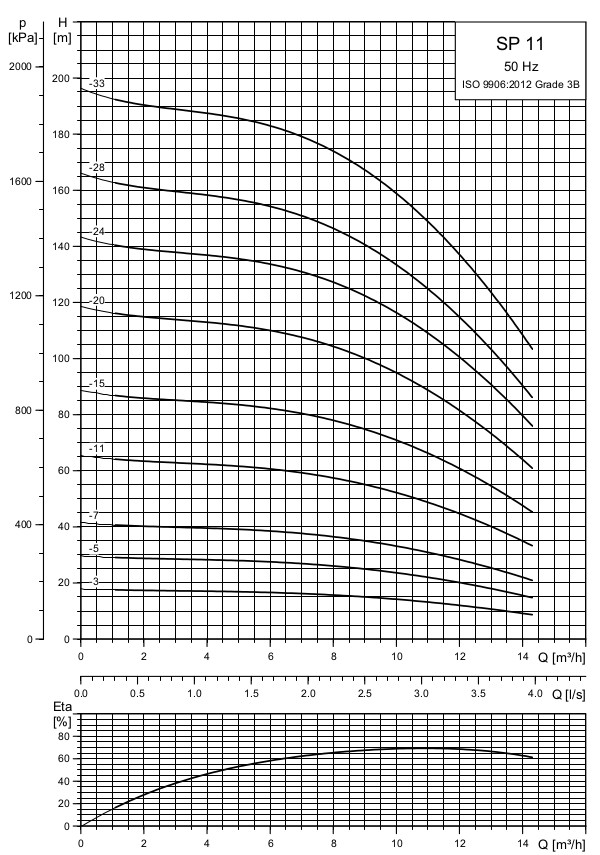
\includegraphics[height=0.8\textheight]{../figs/CurvaSP11.jpg}
\end{column}

\begin{column}{5cm\textwidth}
\begin{itemize}
\item Los catálogos recogen información del funcionamiento instantáneo a frecuencia nominal.
\item Las curvas H-Q no son de uso inmediato para el dimensionado de un SFB.
\end{itemize}
\end{column}
\end{columns}
\end{frame}


\begin{frame}[label=sec-4-3]{Curvas HQ a frecuencia variable}
\begin{itemize}
\item Leyes de la semejanza (rendimiento constante)
\end{itemize}
\begin{align*}
Q &\propto n &H &\propto n^{2}\\
P_{mec} &\propto n^{3} &T &\propto n^{2}
\end{align*}

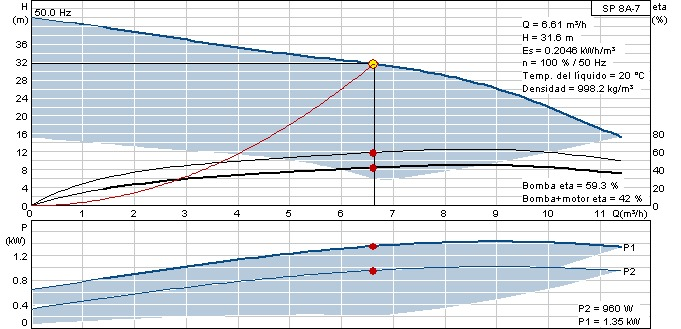
\includegraphics[width=.9\linewidth]{/home/oscar/github/esf/figs/CurvaHQ.png}

\begin{itemize}
\item Para aproximar el funcionamiento en frecuencia variable, es recomendable \alert{multiplicar el valor de $H_{TE}$ por un factor de $1.4$}.
\end{itemize}
\end{frame}

\begin{frame}[label=sec-4-4]{Simulación}
\begin{itemize}
\item Es recomendable simular el funcionamiento del sistema para afinar el dimensionado.
\item El resultado es un gráfico de doble entrada para un modelo concreto de bomba
\end{itemize}
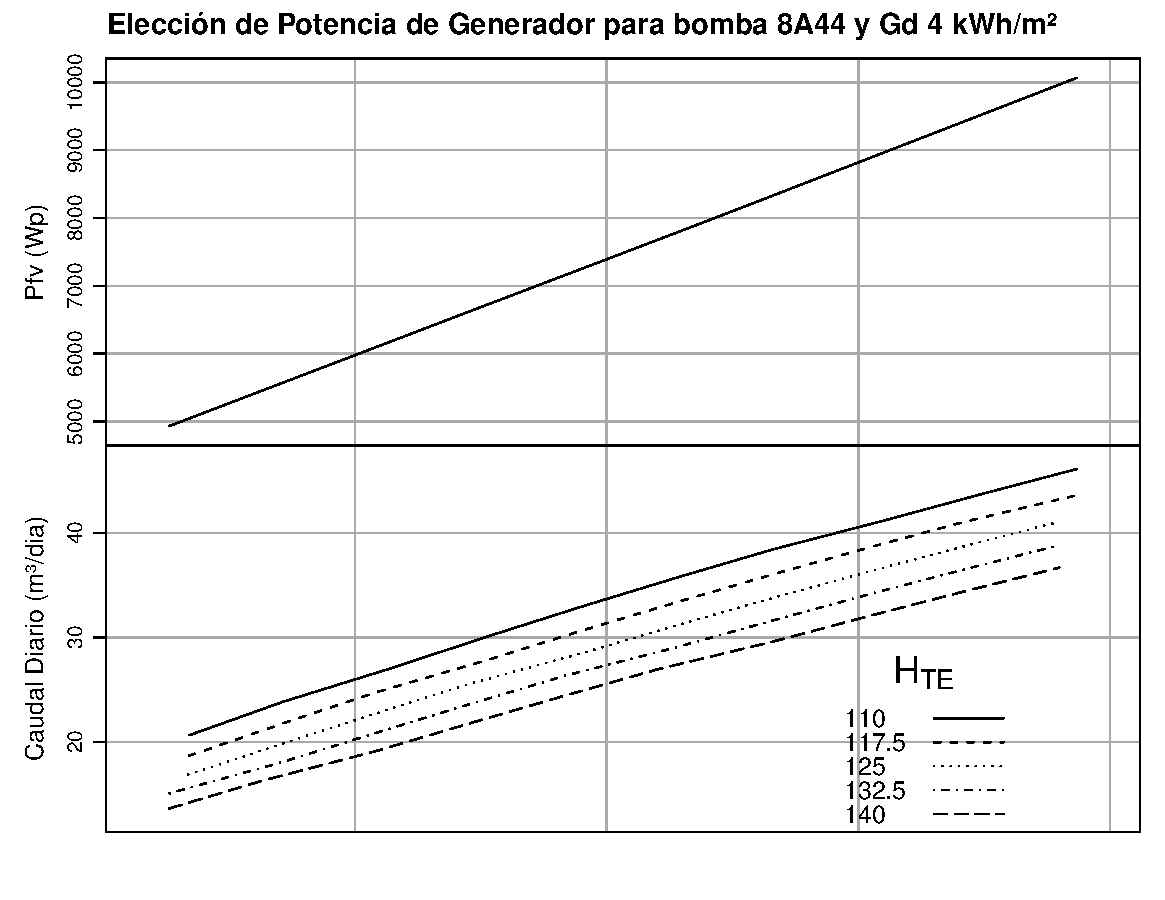
\includegraphics[width=.9\linewidth]{../figs/AbacoBomba.pdf}
\end{frame}

\begin{frame}[label=sec-4-5]{Configuración eléctrica}
\begin{itemize}
\item La tensión de entrada al variador debe ser:$$V_{DC}=\frac{\sqrt{2}V_{AC}}{1.1}$$

\item Para una bomba de tensión de $230\, V_{ac}$ se necesita una tensión en la entrada que no sea inferior a $V_{dc}\simeq300\, V_{dc}$.

\item A partir de esta tensión se configura el número de módulos por serie y el número de ramas del generador.
\end{itemize}
\end{frame}

\begin{frame}[label=sec-4-6]{Pozo, Depósito y Tubería}
\begin{itemize}
\item Como seguridad, cuando la potencia entregada por el generador es igual al 80\% de su potencia nominal, el caudal bombeado correspondiente no debe exceder el máximo admisible por el pozo.
\item El tamaño del depósito será el suficiente para 1 o 2 días de consumo.
\item A partir del caudal $Q_{AP}$ y de la longitud de tubería necesaria, se elige el diámetro de la misma (en curvas del fabricante) de forma que las pérdidas sean inferiores a un porcentaje prefijado de $H_{te}$.
\end{itemize}
\end{frame}
% Emacs 24.4.1 (Org mode 8.2.7c)
\end{document}